\chapter {Resultados}

\section{ANT}
Até a última versão deste projeto, 1.9.5, não foram encontradas utilização métodos com \textit{vargs}, expressões lambdas, \textit{switch} com \textit{strings} e nem \textit{try} com \textit{resources}.\\

Este projeto faz um bom uso de tratamento de exceções sendo encontrado em toda história de desenvolvimento foram produzidas 28 versões deste e com um total de 34722 blocos \textit{trys}, onde em média foram encontradas 1240 destes blocos por versão. E deste total pode-se verificar um total de 513 ocorrências de blocos \textit{trys} com \textit{catchs} iguais totalizando em 1,5\% de código repetido neste quesito conforme ilustra Figura: \ref{fig:TrysAnt}.\\

	\begin{figure}[h]
		\center
		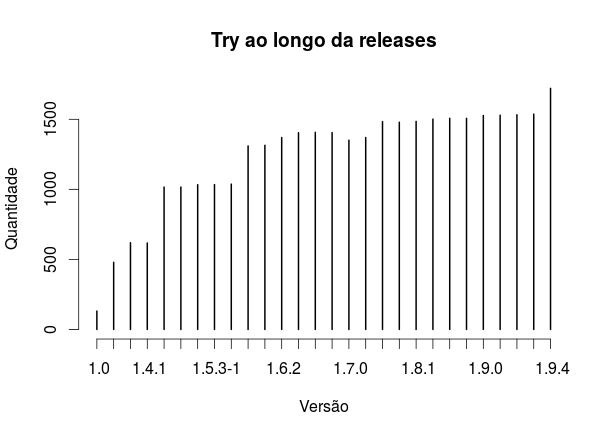
\includegraphics[width=0.7\textwidth]{Imagens/trysAnt}
		\label{fig:TrysAnt}
		\caption{Tratamento de exceção ao longo das releases.}
	\end{figure}

Entretanto pode-se constatar conforme ilustrado na Figura: \ref{fig:catchIguais} que em todas as versões do projeto \textit{ANT} possui o tratamento de exceção como blocos \textit{catchs} iguais sendo contabilizado um total de 513 ocorrências e dando atenção especial entre as versões 1.9.0 e 1.9.5. Entretanto a partir da versão 1.9.0 por volta de 2012, java possuía o mecanismo de \textit{multicatch} que fora lançado por volta de 2011 em java 7. Entre as \textit{releases} desta versão foram encontradas em cada um dos 5 lançamentos do \textit{ANT} por volta de 27 ocorrências iguais de \textit{catchs} e acarreta em um total de 135 blocos repetidos. Caso fosse adotado \textit{multicatch} seria reduzido somente a 5 blocos a cada versão existente o que seria uma redução de código repetido em aproximadamente 18\%, e isso acarretaria em um código mais atual e elegante.\\

	\begin{figure}[h]
		\center
		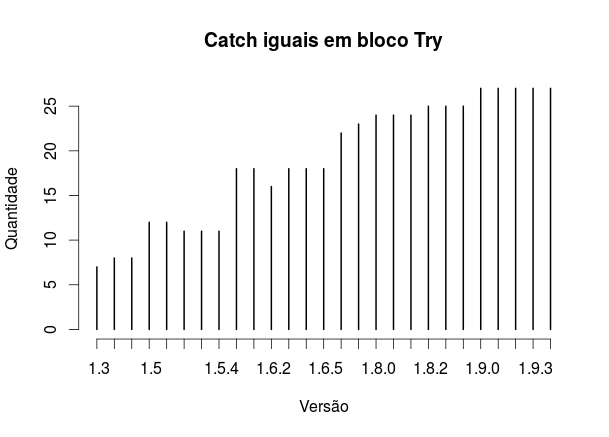
\includegraphics[width=0.7\textwidth]{Imagens/catchsIguais}
		\label{fig:catchIguais}
		\caption{Bloco Try com catchs iguais ao longo das releases.}
	\end{figure}
